\documentclass[10pt,a4paper]{article}
\usepackage[utf8]{inputenc}
\usepackage[T1]{fontenc}
\usepackage[margin=20mm]{geometry}
\usepackage{amsmath,amssymb}
\usepackage{graphicx}
\usepackage{booktabs}
\usepackage{array}
\usepackage{longtable}
\usepackage[table,dvipsnames]{xcolor}
\usepackage[font=small,labelfont=bf]{caption}
\usepackage{hyperref}
\usepackage{fancyhdr}
\usepackage{enumitem}
\usepackage{float}

\definecolor{hdrblue}{HTML}{2F6FB5}
\definecolor{rowlt}{HTML}{EFF3F8}
\hypersetup{colorlinks=true,linkcolor=hdrblue,urlcolor=hdrblue}
\setlist{itemsep=1pt,topsep=3pt}
\setlength{\parskip}{4pt}
\setlength{\parindent}{0pt}
\newcommand{\hdr}[1]{\textcolor{white}{\textbf{#1}}}
\pagestyle{fancy}
\fancyhf{}
\fancyhead[R]{\small\thepage}
\renewcommand{\headrulewidth}{0.4pt}

\newcommand{\pbstartcycle}{239.8}
\newcommand{\pbstartviol}{28}
\newcommand{\pbstartjoints}{8911.0}
\newcommand{\pbstartpath}{15.7}
\newcommand{\pbstartmoves}{120}
\newcommand{\pbbestcycle}{112.9}
\newcommand{\pbbestviol}{0}
\newcommand{\pbbestjoints}{3670.0}
\newcommand{\pbbestpath}{7.82}
\newcommand{\pbbestmoves}{84}
\newcommand{\pbbestit}{30}
\newcommand{\pbniter}{30}
\newcommand{\pbnkept}{29}
\newcommand{\pbnrej}{1}
\newcommand{\pbcost}{41}
\newcommand{\pbagentmin}{106}
\newcommand{\pbtstart}{2026-11-20 14:40:34}
\newcommand{\pbtend}{2026-11-20 16:27:52}
\newcommand{\pbnlessons}{30}
\newcommand{\pbnagain}{10}
\newcommand{\pbfirstlegal}{8}
\newcommand{\pbgainpct}{53}

\fancyhead[L]{\small MMA4002 DAM -- Assembly experiment, Part B (blind AI run from v3)}

\title{\vspace{-14mm}\textbf{Assembly experiment, Part B}\\[1mm]
\large A blind AI agent improves the bench cell from v3 --- what it did, why, and what it learnt}
\author{Bjørge (report written by Claude from the run logs)}
\date{Run: \pbtstart{} -- \pbtend{} on bj-hserver \quad Report: 2026-11-22}

\begin{document}
\maketitle
\thispagestyle{fancy}

\section*{Summary}
Starting from the first working bench cell (\textbf{v3}: \pbstartcycle{}\,s, \pbstartviol{} hard-rule violations), a
headless Claude agent working blind (no access to our later versions) ran \pbniter{} iterations in about 1 h 47 min
of wall time and reached a \textbf{legal cell at \pbbestcycle{}\,s} (iter \pbbestit{}), \textbf{\pbgainpct{}\,\% faster}
than v3, with joint travel \pbstartjoints{} $\to$ \pbbestjoints{}\,deg and TCP path \pbstartpath{} $\to$ \pbbestpath{}\,m.
It made the cell legal first (iter \pbfirstlegal{}, at a small time cost), then cut time almost only through
program changes. One change dominates: \textbf{dropping the guide's trip to base A and back} (iter 25, $-47.5$\,s).
\pbnkept{} of \pbniter{} iterations were kept, \pbnrej{} rejected. It logged \pbnlessons{} lessons
(\pbnagain{} of them marked as a repeat of an earlier lesson), built 25 of its own tools, and proposed one fix to
the judge (a Line's time ignored tool rotation), which is applied in run B2. Cost: about \$\pbcost{} of API use,
\pbagentmin{} min of agent time. The run stopped because it hit the 30-iteration cap, \emph{not} because it ran out
of ideas: the last kept change was iteration 30.

\section{What was tested}
\begin{itemize}
\item \textbf{Question:} from v3, how far can an AI agent improve the automated assembly with our own simulation tools
  (no RoboDK), and what kind of changes does it find?
\item \textbf{Setup:} a sandbox on bj-hserver with v3's program and cell, the jig/bench CAD scripts and a
  \textbf{frozen judge} (collision, kinematics, cycle time, manipulability; SHA-256 checked every minute). A
  leak check made sure no later design ideas (v4--v10) were in the sandbox. One headless \texttt{claude -p}
  session per iteration with \texttt{AGENT.md} as its brief.
\item \textbf{It could change:} the program, the jig layout, the jig CAD (build123d), and its own tools. Not the
  speeds, gripper, robot, TCP or the bench product.
\item \textbf{Hard rules} (any violation = reject): r1 no collisions (2\,mm sampling), r2 reachable, r3 last/first
  50\,mm vertical and slow, r4 no PTP near parts, r5 clearance $\ge$10\,mm, r6 released parts rest on something,
  r7 jigs printable and on the plate, r8 bench assembled at the end.
\item \textbf{Keep rule:} rank $=$ (fails a rule?, violations, cycle time, joint travel), lower is better.
  Budget: 30 iterations, stop after 5 in a row without a keep.
\item \textbf{Per iteration} the agent had to write a hypothesis with the expected $\Delta$ \emph{before} scoring,
  look at the rendered screenshots before keeping, and log every problem as a lesson.
\end{itemize}

\section{Result}
\begin{table}[H]
\centering\small
\rowcolors{2}{rowlt}{white}
\begin{tabular}{l r r l}
\toprule
\rowcolor{hdrblue}\hdr{Metric} & \hdr{v3 (iter 00)} & \hdr{Best (iter \pbbestit)} & \hdr{Note}\\
\midrule
Cycle time, programmed speeds & \pbstartcycle\,s & \pbbestcycle\,s & $-$\pbgainpct\,\%\\
Cycle time with ramps & 270.9\,s & 135.0\,s & trapezoid estimate\\
Hard-rule violations & \pbstartviol & \pbbestviol & r1 5, r3 18, r4 1, r5 4 $\to$ 0\\
Joint travel (sum J1--J6) & \pbstartjoints\,deg & \pbbestjoints\,deg & J6 1656 $\to$ 329, J1 593 $\to$ 189\\
TCP path & \pbstartpath\,m & \pbbestpath\,m & \\
Moves (PTP / Line) & 120 (22 / 98) & 84 (18 / 66) & \\
Grips & 9 & 7 & guide grips gone\\
Min clearance in free moves & 3.0\,mm & 41.5\,mm & rule: $\ge$10\,mm\\
\bottomrule
\end{tabular}
\caption{Start vs best, both scored by the same frozen judge at 2\,mm.}
\end{table}

\begin{figure}[H]
\centering
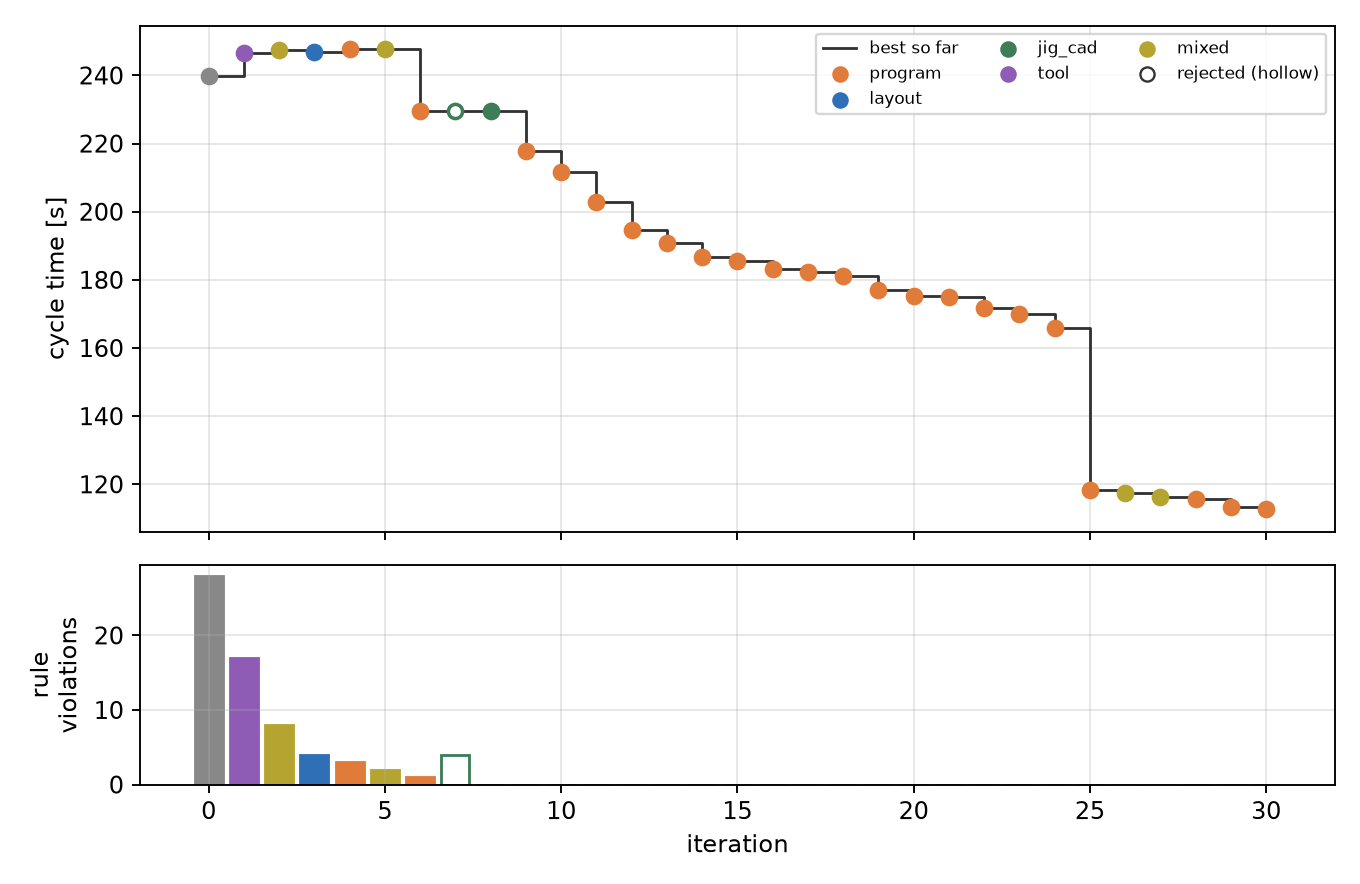
\includegraphics[width=.86\linewidth]{part_b/fig_progress.png}
\caption{Every iteration (filled = kept, hollow = rejected, colour = change type) and the best so far. Iterations
1--8 trade a little time for legality; 9--24 are steady program tuning; 25 removes the guide trip.}
\end{figure}

\begin{figure}[H]
\centering
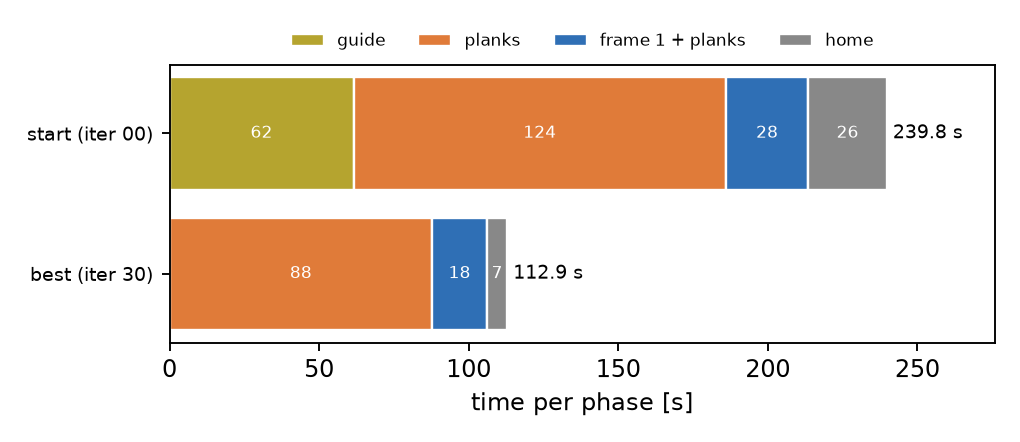
\includegraphics[width=.72\linewidth]{part_b/fig_phases.png}
\caption{Where the time goes. The guide phase disappears; the planks phase is now ~74\,\% fixed cost
(50\,mm slow legs at 20\,mm/s and gripper waits), which is why later gains get small.}
\end{figure}

\begin{figure}[H]
\centering
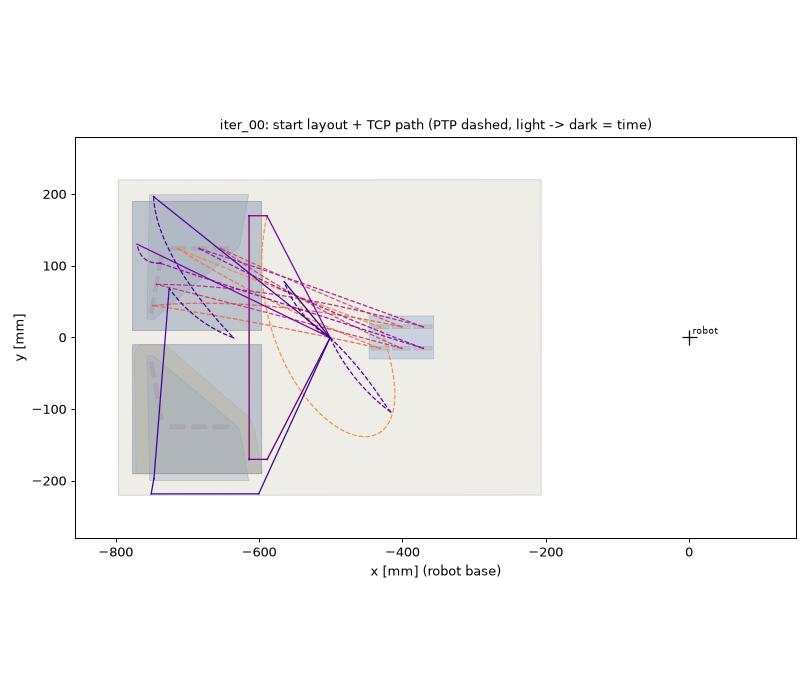
\includegraphics[width=.49\linewidth]{../results/part_b/log/iter_00/topview.png}\hfill
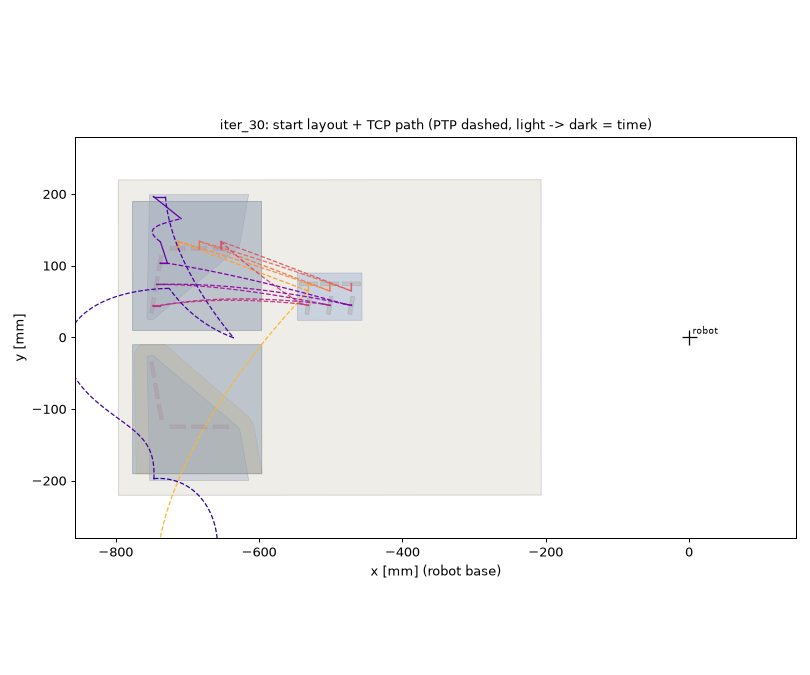
\includegraphics[width=.49\linewidth]{../results/part_b/log/iter_30/topview.png}
\caption{Top view with the TCP path: v3 (left) and the best design (right). The long guide carries between base B
and base A are gone, and the plank jig sits closer to base A.}
\end{figure}

\section{What it changed, and why}
Part B's brief asked for a \emph{hypothesis} per iteration (what, why, expected $\Delta$), not a separate reason
section; the reasons below are condensed from those hypotheses (\texttt{results/part\_b/log/iter\_NN/notes.md}). In
run B2 a written \texttt{Reason} is a hard rule and goes into the iteration log.

\begin{figure}[H]
\centering
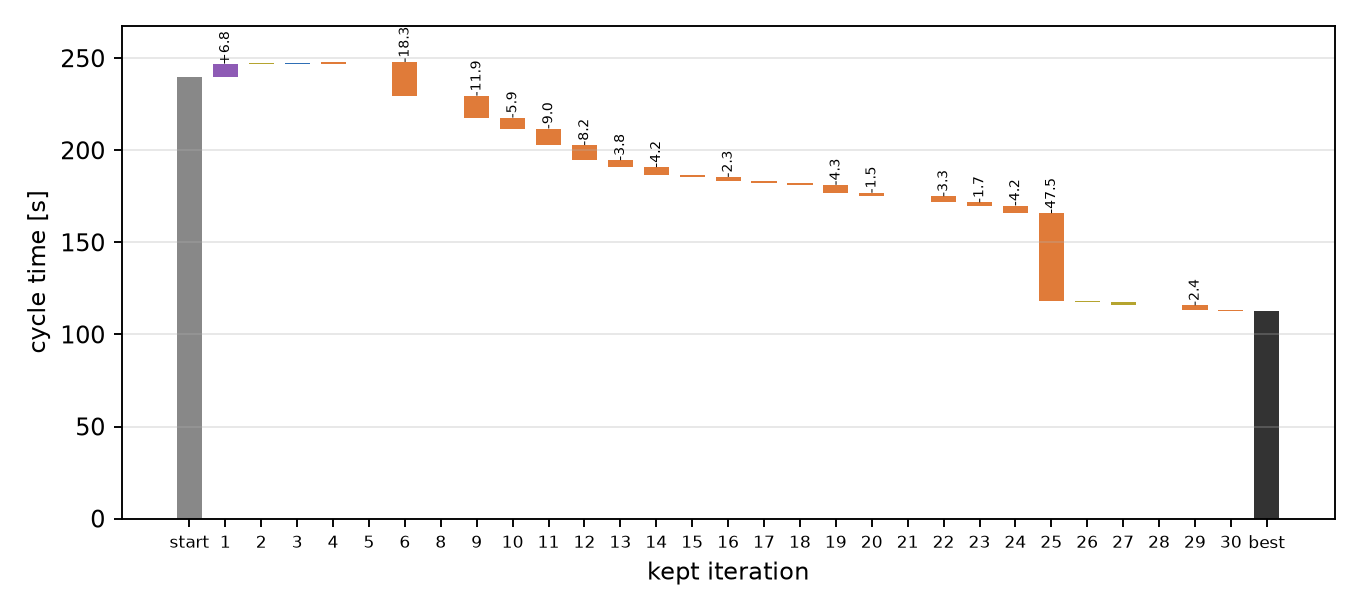
\includegraphics[width=.86\linewidth]{part_b/fig_waterfall.png}
\caption{Waterfall of kept changes (bar = $\Delta$ cycle time, colour = change type). Iterations 1--5 add time
(making it legal); iteration 25 is the big step.}
\end{figure}

{\small
\rowcolors{2}{rowlt}{white}
\begin{longtable}{>{\raggedleft}p{5mm} p{12mm} >{\raggedright}p{85mm} r r r p{14mm}}
\toprule
\rowcolor{hdrblue}\hdr{It} & \hdr{Type} & \hdr{Change and reason} & \hdr{Cycle} & \hdr{$\Delta$s} & \hdr{Viol.} & \hdr{Result}\\
\midrule
\endhead
1 & tool & \textbf{slow vertical 50 mm approach/retreat at every grip/release (tool)}\newline Why: 12 of v3's 18 approach violations (r3) were slow vertical legs shorter than 50 mm; one tool fixes all of that kind at once. Accepted +6.8 s, because legal comes before fast. & 246.6 & +6.8 & 17 & kept \\
2 & mixed & \textbf{guide gripped from above - grip pocket becomes a vertical through-notch (mixed: jig\_cad + program)}\newline Why: 4 of the remaining 6 r3 hits were the guide's sideways slide into its closed side pocket. A vertical through-notch allows a grip from above (DFA: top-down handling). CAD + program together, because neither half works alone. & 247.5 & +0.9 & 8 & kept \\
3 & layout & \textbf{plank jig moved 60 mm toward base A (layout + plank-pick moves shifted)}\newline Why: 5 of 8 violations were the forearm (link 3) hitting planks 4/5 in the jig while it reached for the guide on base B. Moving the jig 60 mm away from that reach removes the cause instead of re-routing around it. & 247.0 & -0.5 & 4 & kept \\
4 & program & \textbf{frame lift-out PTP (Point82) $\to$ fast Line}\newline Why: r4 flagged the PTP lift-out starting only 50 mm above the frame grip. Both ends have the same tool orientation, so a straight Line rises vertically and is legal. & 247.9 & +0.9 & 3 & kept \\
5 & mixed & \textbf{raise the plank1 transit (Point56) so plank1 clears plank2}\newline Why: the carried plank1 swept through the top of the already placed plank2 (r1). Measured it first (L07): needed more transit height, not a new route. & 247.9 & +0.0 & 2 & kept \\
6 & program & \textbf{vertical exit out of the frame release}\newline Why: the exit after the frame release was a slow sideways dogleg ($\sim$18 s at 20 mm/s, and an r3 hit). Leaving straight up the way it came in removes both. & 229.6 & -18.3 & 1 & kept \\
7 & jig\_cad & \textbf{relief recesses under the plank ends in base B}\newline Why: the last violation was a zero-depth contact of the plank ends on the base B pocket floor. A 2 mm relief under the plank ends should remove it. Rejected: it also removed the floor under 4 interface pieces (r6). & 229.6 & +0.0 & 4 & rejected \\
8 & jig\_cad & \textbf{plank-end relief in base B that keeps the floor under the pieces B}\newline Why: iter 07's idea was right but the cut was too wide. Cut only the plank-end footprints minus the interface-piece footprints. First legal design. & 229.6 & +0.0 & 0 & kept \\
9 & program & \textbf{drop the redundant plank push after every plank release}\newline Why: biggest phase = planks (127 s). The push after each release (close, push 20 mm, open) moved nothing: the release pose was already home (r8 still passes). Remove a whole handling step x6. & 217.7 & -11.9 & 0 & kept \\
10 & program & \textbf{shorten the slow plank-place descent from 75 to 50.5 mm}\newline Why: the place descent was slow for 75 mm but the rule needs only the last 50 mm slow; 25 mm at 20 mm/s $\to$ at 100 mm/s saves $\sim$1 s per plank. & 211.8 & -5.9 & 0 & kept \\
11 & program & \textbf{outbound guide transfer with PTPs instead of long 100 mm/s Lines}\newline Why: guide phase (62 s) was long 100 mm/s Lines; a PTP over the same distance is faster (joint speed). Outbound transfer first. & 202.8 & -9.0 & 0 & kept \\
12 & program & \textbf{return guide transfer with PTPs instead of long 100 mm/s Lines}\newline Why: same evidence and change as iter 11, for the return transfer ($\sim$22 s of Lines). & 194.6 & -8.2 & 0 & kept \\
13 & program & \textbf{lower the plank transit points from TCP z 391 to grip/release + 102.5 mm}\newline Why: every plank pick/place went through a transit at TCP z 391 although the rules only need $\sim$100 mm clearance; lower transits shorten 24 fast Lines. & 190.8 & -3.8 & 0 & kept \\
14 & program & \textbf{frame-1 approach with one PTP + vertical Line instead of the Lines via (-500, 0)}\newline Why: the frame-1 approach was 11.5 s of Lines and small PTPs via a detour; one PTP + one Line covers it. & 186.6 & -4.2 & 0 & kept \\
15 & program & \textbf{retreat after the frame release as Line up + one PTP}\newline Why: the retreat after the frame release was 3 Lines + a PTP (5.7 s); Line up + one PTP is shorter. & 185.5 & -1.1 & 0 & kept \\
16 & program & \textbf{plank pick slow lift 60 $\to$ 50.5 mm}\newline Why: still biggest phase planks; the slow lift after each plank grip was 60 mm where 50.5 mm is enough (same logic as iter 10, on the pick side). & 183.2 & -2.3 & 0 & kept \\
17 & program & \textbf{frame release slow leg 75 $\to$ 50.5 mm}\newline Why: same 75 $\to$ 50.5 mm slow-leg cut for the frame release. & 182.2 & -1.0 & 0 & kept \\
18 & program & \textbf{lift after the guide release on base A as a short vertical Line + the existing PTP}\newline Why: after releasing the guide the arm climbed to z 461, a height left over from v3's route; climb only as high as the next PTP needs. & 181.2 & -1.0 & 0 & kept \\
19 & program & \textbf{J6 unwrapped +360 deg from the guide flip to the plank6 pick and over the guide return}\newline Why: the longest PTP was J6-bound (232 deg); unwrapping J6 by +360 deg keeps the same pose with a shorter turn (lowering a PTP was tried first in screens and dropped, L19). & 176.9 & -4.3 & 0 & kept \\
20 & program & \textbf{guide return grip at J6 +180 (short way from plank4), lift Point11r higher so the opposite flip clears}\newline Why: the guide return grip turned J6 the long way from plank4; grip at J6 +180 and lift higher so the opposite flip clears plank6. & 175.4 & -1.5 & 0 & kept \\
21 & program & \textbf{guide placement on base A: PTP end Point11h offset sideways and lower, short diagonal Line down}\newline Why: a 244 mm Line dropped the guide straight down only because the PTP end had to stay 100 mm from a plank release point; move that PTP end sideways instead of up. & 175.0 & -0.4 & 0 & kept \\
22 & program & \textbf{plank transits offset sideways out of the plank's thin xy box, lowered to event + 102}\newline Why: plank transits sat at +117.5 mm because they were inside the plank's thin (5 mm) xy box; a 10 mm side offset leaves the box and lets them drop to +102 mm (24 Lines shorter). & 171.7 & -3.3 & 0 & kept \\
23 & program & \textbf{guide-grip transits over base A (Point15v, Point14h) offset sideways and lowered}\newline Why: same side-offset idea for the guide-grip transits over base A (long 240 mm vertical Lines). & 170.0 & -1.7 & 0 & kept \\
24 & program & \textbf{home pose moved onto the joint path between the last release lift and the first guide approach}\newline Why: start/end of the cycle cost 4 s of wrist-branch (J5) swings; put home on the joint path between the last lift and the first approach. & 165.8 & -4.2 & 0 & kept \\
25 & program & \textbf{the guide stays on base B (no guide trip to base A and back)}\newline Why: the guide's trip to base A and back ($\sim$46 s) only serves as a placing aid; frame 1 already holds the planks upright alone, and no rule needs the trip. Lesson L25: question whether a phase is needed before tuning it. & 118.3 & -47.5 & 0 & kept \\
26 & mixed & \textbf{plank jig moved toward base A (shorter pick $<$$\to$ place PTPs)}\newline Why: with the guide trip gone, the gap between plank jig and base A was free; moving the jig closer shortens 12 pick/place PTPs (got less than expected: those PTPs were J6-bound). & 117.5 & -0.8 & 0 & kept \\
27 & mixed & \textbf{planks 4-6 presented pre-rotated 80 deg in the jig, placed as a group after 3, 1, 2}\newline Why: five PTPs were J6-bound because planks 4-6 sit 80 deg turned in the frame vs the jig; present them pre-rotated (DFA: present parts in assembly orientation) and place them as a group. & 116.2 & -1.3 & 0 & kept \\
28 & program & \textbf{frame flip as one PTP onto the other wrist branch (short return home)}\newline Why: the end of the cycle was set by a 228 deg J5 swing; a PTP flip onto the other wrist branch (a Line could not, L24) shortens the return home. & 115.8 & -0.4 & 0 & kept \\
29 & program & \textbf{frame-grip approach PTP ends further down the diagonal Line (short Line)}\newline Why: the 320 mm diagonal Line to the frame-foot grip was the longest single move left; end the PTP further down it. & 113.4 & -2.4 & 0 & kept \\
30 & program & \textbf{shorter fast lift Point80u $\to$ Point80L after the frame-foot grip}\newline Why: the lift after the frame grip climbed higher than r4 needs before the flip PTP; stop it lower (small, -0.5 s). & 112.9 & -0.5 & 0 & kept \\
\bottomrule
\end{longtable}
}


\subsection*{Patterns in its reasoning}
\begin{itemize}
\item \textbf{Legal first, then fast.} Iterations 1--8 each fixed the biggest group of violations, even when that
  cost time (+8.1\,s over iterations 1--5, before iter 6 won it back). That follows the keep rule exactly.
\item \textbf{Biggest phase first.} From iter 9 it attacked the largest phase (planks, then guide) and said so in
  each hypothesis.
\item \textbf{Mostly small, safe program edits.} 22 of 30 iterations were program-only; it made only 2 jig-CAD
  changes, 1 layout move, 4 mixed changes and 1 pure tool change, so the cell's \emph{design} changed little.
\item \textbf{The big win came late.} The guide trip (iter 25) was questioned only after 24 iterations of tuning the
  moves inside it. Its own lesson L25 says it: ask whether a phase is needed before tuning it. A human DFA review
  would ask that first.
\item \textbf{Its predictions were good.} Most results landed within a few tenths of a second of the expected
  $\Delta$; where they missed (iter 13, 26, 27) it found and logged the cause (a stricter r4 box, J6-bound PTPs).
\end{itemize}

\section{What it learnt (lessons log)}
The agent wrote a lesson block (problem, cause, fix, rule) at once for every problem, re-read the log at the start of
every iteration, and copied 12 lessons into \texttt{AGENT.md} as standing rules.

\begin{table}[H]
\centering\small
\rowcolors{2}{rowlt}{white}
\begin{tabular}{>{\raggedright}p{38mm} >{\raggedright}p{22mm} >{\raggedright\arraybackslash}p{95mm}}
\toprule
\rowcolor{hdrblue}\hdr{Kind} & \hdr{Lessons} & \hdr{Typical rule it learnt}\\
\midrule
Judge checks and margins & L01, L03, L14, L15, L22, L30 & Never aim at a threshold exactly (50.5\,mm legs); the 10\,mm screen misses thin-part r4 hits, screen at 2\,mm; read how the judge times a move before targeting it.\\
PTP planning near parts & L13, L17, L23, L25, L27, L29 & Both ends of every PTP $\ge$100\,mm from \emph{all} grip/release points; a just-released part is an obstacle; fix a PTP-end hit by moving its start.\\
Robot arm and wrist & L04, L06, L16, L19--L21, L24, L26, L28 & A PTP end lowers the whole swing (check the wrist mid-swing); probe IK and wrist branches before a change; J6 $\pm$360 keeps the pose.\\
Parts and jig geometry & L05, L07, L09, L10, L12 & Measure a contact before fixing it; the judge's meshes are the truth, not the STEP; before cutting a jig surface, list every part that rests on it.\\
Its own working environment & L02, L08, L11, L18 & Edit files with Edit/Write, one \texttt{./py} per call; append to logs with Edit, never overwrite (L18: it wiped its lessons once).\\
\bottomrule
\end{tabular}
\caption{The 30 lessons grouped by kind.}
\end{table}

\textbf{Did it actually learn?} Partly. \pbnagain{} of the 30 lessons are marked as a repeat of an earlier one.
The repeats cluster in two places: the sandbox's shell permissions (L02 again in L08 and L11: it kept trying
chained or inline shell commands), and the r4 ``thin box'' over planks (L15, L22, L23 again in L25, L27, L29).
For the first, the lesson stuck after the third time. For the second, each repeat was a \emph{new variant} of the same
geometry trap (start vs end of the PTP, after a rotation), and each was caught by the 2\,mm score, never kept. So
the lessons log worked as a safety net and a memory, but rules phrased for one case did not always transfer to the
next case.

\textbf{Tools it built.} 25 tool blocks in \texttt{tool\_changes.md} (e.g. \texttt{slow\_approach.py},
\texttt{lower\_transit.py}, \texttt{side\_transit.py}, \texttt{home\_on\_path.py}, \texttt{j6\_wrap.py},
\texttt{drop\_range.py}): each is a small program transformer, so every change is reproducible from the previous
program. It also proposed one \textbf{judge fix}: a Line's time was its TCP distance only, so a pure re-orientation
costs 0\,s. It noted that it did not exploit it. The fix is applied in B2 (+2.0\,s on this design).

\section{Caveats for the DAM report}
\begin{itemize}
\item \textbf{The guide is no longer used as a placing aid.} Frame 1 already holds the planks upright alone in v3's
  later steps, and no rule says the guide must visit base A, so the agent dropped the trip. On the real cell the
  planks then go into frame 1 on robot accuracy alone; a trial insertion (or a cheap fixed guide on base A) should
  confirm it. This is a real process trade-off, not just a faster program.
\item \textbf{Simulated time only:} programmed speeds, no blending, no controller limits beyond the judge's model.
\item \textbf{Not comparable to our own v4--v10 path in time:} our versions added functions (vision-found layout,
  other gripper, two benches), and v10 scores 295.9\,s under Part A rules. The fair comparison is v3 $\to$ best
  under one judge.
\item \textbf{Blindness held:} the only ``outside'' file accesses (7 \texttt{leak\_risk} events) were the agent
  reading its own large tool outputs in Claude's temp folder; the permissions denied those reads.
\end{itemize}

\section*{Files}
Logs: \texttt{results/part\_b/log/} (\texttt{iterations.csv}, \texttt{iter\_NN/notes.md}, \texttt{lessons.md},
\texttt{tool\_changes.md}, \texttt{summary.md}, \texttt{run.jsonl}); best design: \texttt{results/part\_b/best/};
figures: \texttt{report/build\_figs.py part\_b}.

\end{document}
